\chapter{Class notes} 
\includepdf[pages={53-61}]{sources/polyEDP-M1-main.pdf}

\chapter{Ordinary Differential Equations} 
\section{Elementary Integration Methods}
\label{sec:Elementary Integration Methods}
\subsection{First Order Equations}
\label{subsec:First Order Equations}
\subsubsection{Seperable Variables}
Consider
\begin{equation}
    y '= f(x) g(y)      
    \label{eq:seperable}
\end{equation}
can be serperated and divided such that 
\[
\int\limits_{ }^{ } \frac{ dy }{ g(y)  } = \int\limits_{ }^{ } f(x) \ dx + C
\]
A special case of this is $ y'= f(x) y $, which has solution 
\[
    y(x) = CR(x) , \qquad R(x) = exp\left( \int\limits_{ }^{ } f(x) \ dx\right) 
\]

\subsubsection{Inhomogeneous Linear Equation}
\begin{equation}
    y ' =  f(x) y + g(x) 
    \label{eq:inhomoLineq}
\end{equation}
Then the solution is given by 
\[
    y = e _{  }^{ - \int\limits_{ }^{ } f(x)\  dx    } \left( C + \int\limits_{ }^{ } g(x)
    e _{  }^{ \int\limits_{ }^{ } f(x) \ dx } \ dx\right)  
\]


\subsection{Linear Differential Equations}
\label{subsec:Linear Differential Equations}
\subsubsection{Equations with Constant Coefficients}
\begin{equation}
    y _{  }^{ (n) } (x) = 0
    \label{eq:constCoefHomo}
\end{equation}
Integrating n times gives 
\[
    y(x) = C_1x^{n-1} +C_2x^{n-2} + \cdots + C_{n}  
\]
The general equation with constant coefficients is  
\[
    y _{  }^{ (n)  } + A_{n-1}y _{  }^{ (n-1) } + \dots + A_0y = 0
\]

